\chapter{Application}
\label{ch:application}
In this chapter, we describe how we leveraged the time series forecasting techniques
described in the previous chapter to predict earthquakes. We wrap our forecasting
model in a web application and enrich the dashboard with an AI assistant
to enable human-like interactions with the forecasting results.

Together, the dashboard (Appendix Figure \ref{fig:dashboard}) and
AI assistant (Appendix Figure \ref{fig:copilot}) aim at improving our ability to forecast
earthquakes and prepare for their consequences. This chapter explores the functionalities,
underlying technologies, and real-world applications of these tools, highlighting their
potential to revolutionize earthquake forecasting and enhance public safety.

Within the web application there are two main workflows, the first one being an overview and
analysis of recent earthquakes and the second being a conversation with a copilot to
support insights and decision making. Screenshots of the application can be found in
Appendix \ref{ch:web-application-design}.

\section{Modeling Problem}

As earthquakes are not equally distributed over the surface of the earth,
we decided to forecast earthquakes for the 25 most endangered regions on
the planet. This facilitates the forecasting process while only marginally
reducing our use case. To fulfill our goal of warning people about potential
dangers we effectively need to forecast the magnitude, depth and location of
an upcoming earthquake. A reliable prediction of these three features would
enable users to evaluate their situation and take preliminary action if needed.

We have chosen to forecast only the magnitude and depth of earthquakes and
to use historical median values for the location. This decision is based
on the fact that most earthquakes occur at the edges of tectonic plates,
resulting in similar location values for earthquakes within a given region.
By removing the location values as a forecasting target, the modeling problem
becomes more computationally efficient.

\subsection{Data}
To forecast, we utilized data from the \ac{USGS} Earthquake Catalog, accessed via
the \ac{FDSN} Event Web Service. This service provides comprehensive information
on seismic events using various parameters such as time, location, depth, and magnitude.
We queried the catalog for earthquakes from the past 100 years. Due to
limited data prior 1970, we opted to use the data from the past 30 years
for training (Figure \ref{fig:world-map}). Given our focus on building an end-to-end machine learning
application, we opted to use this free API, which allows us to forecast
future earthquakes based on live data. This approach closely resembles a
production system, enhancing the realism and practicality of our forecasting
model. The dataset, available in formats such as GeoJSON, XML, and CSV, was
instrumental in analyzing seismic activity trends and developing the forecasting model.


\begin{figure}[hbtp]
  \centering
  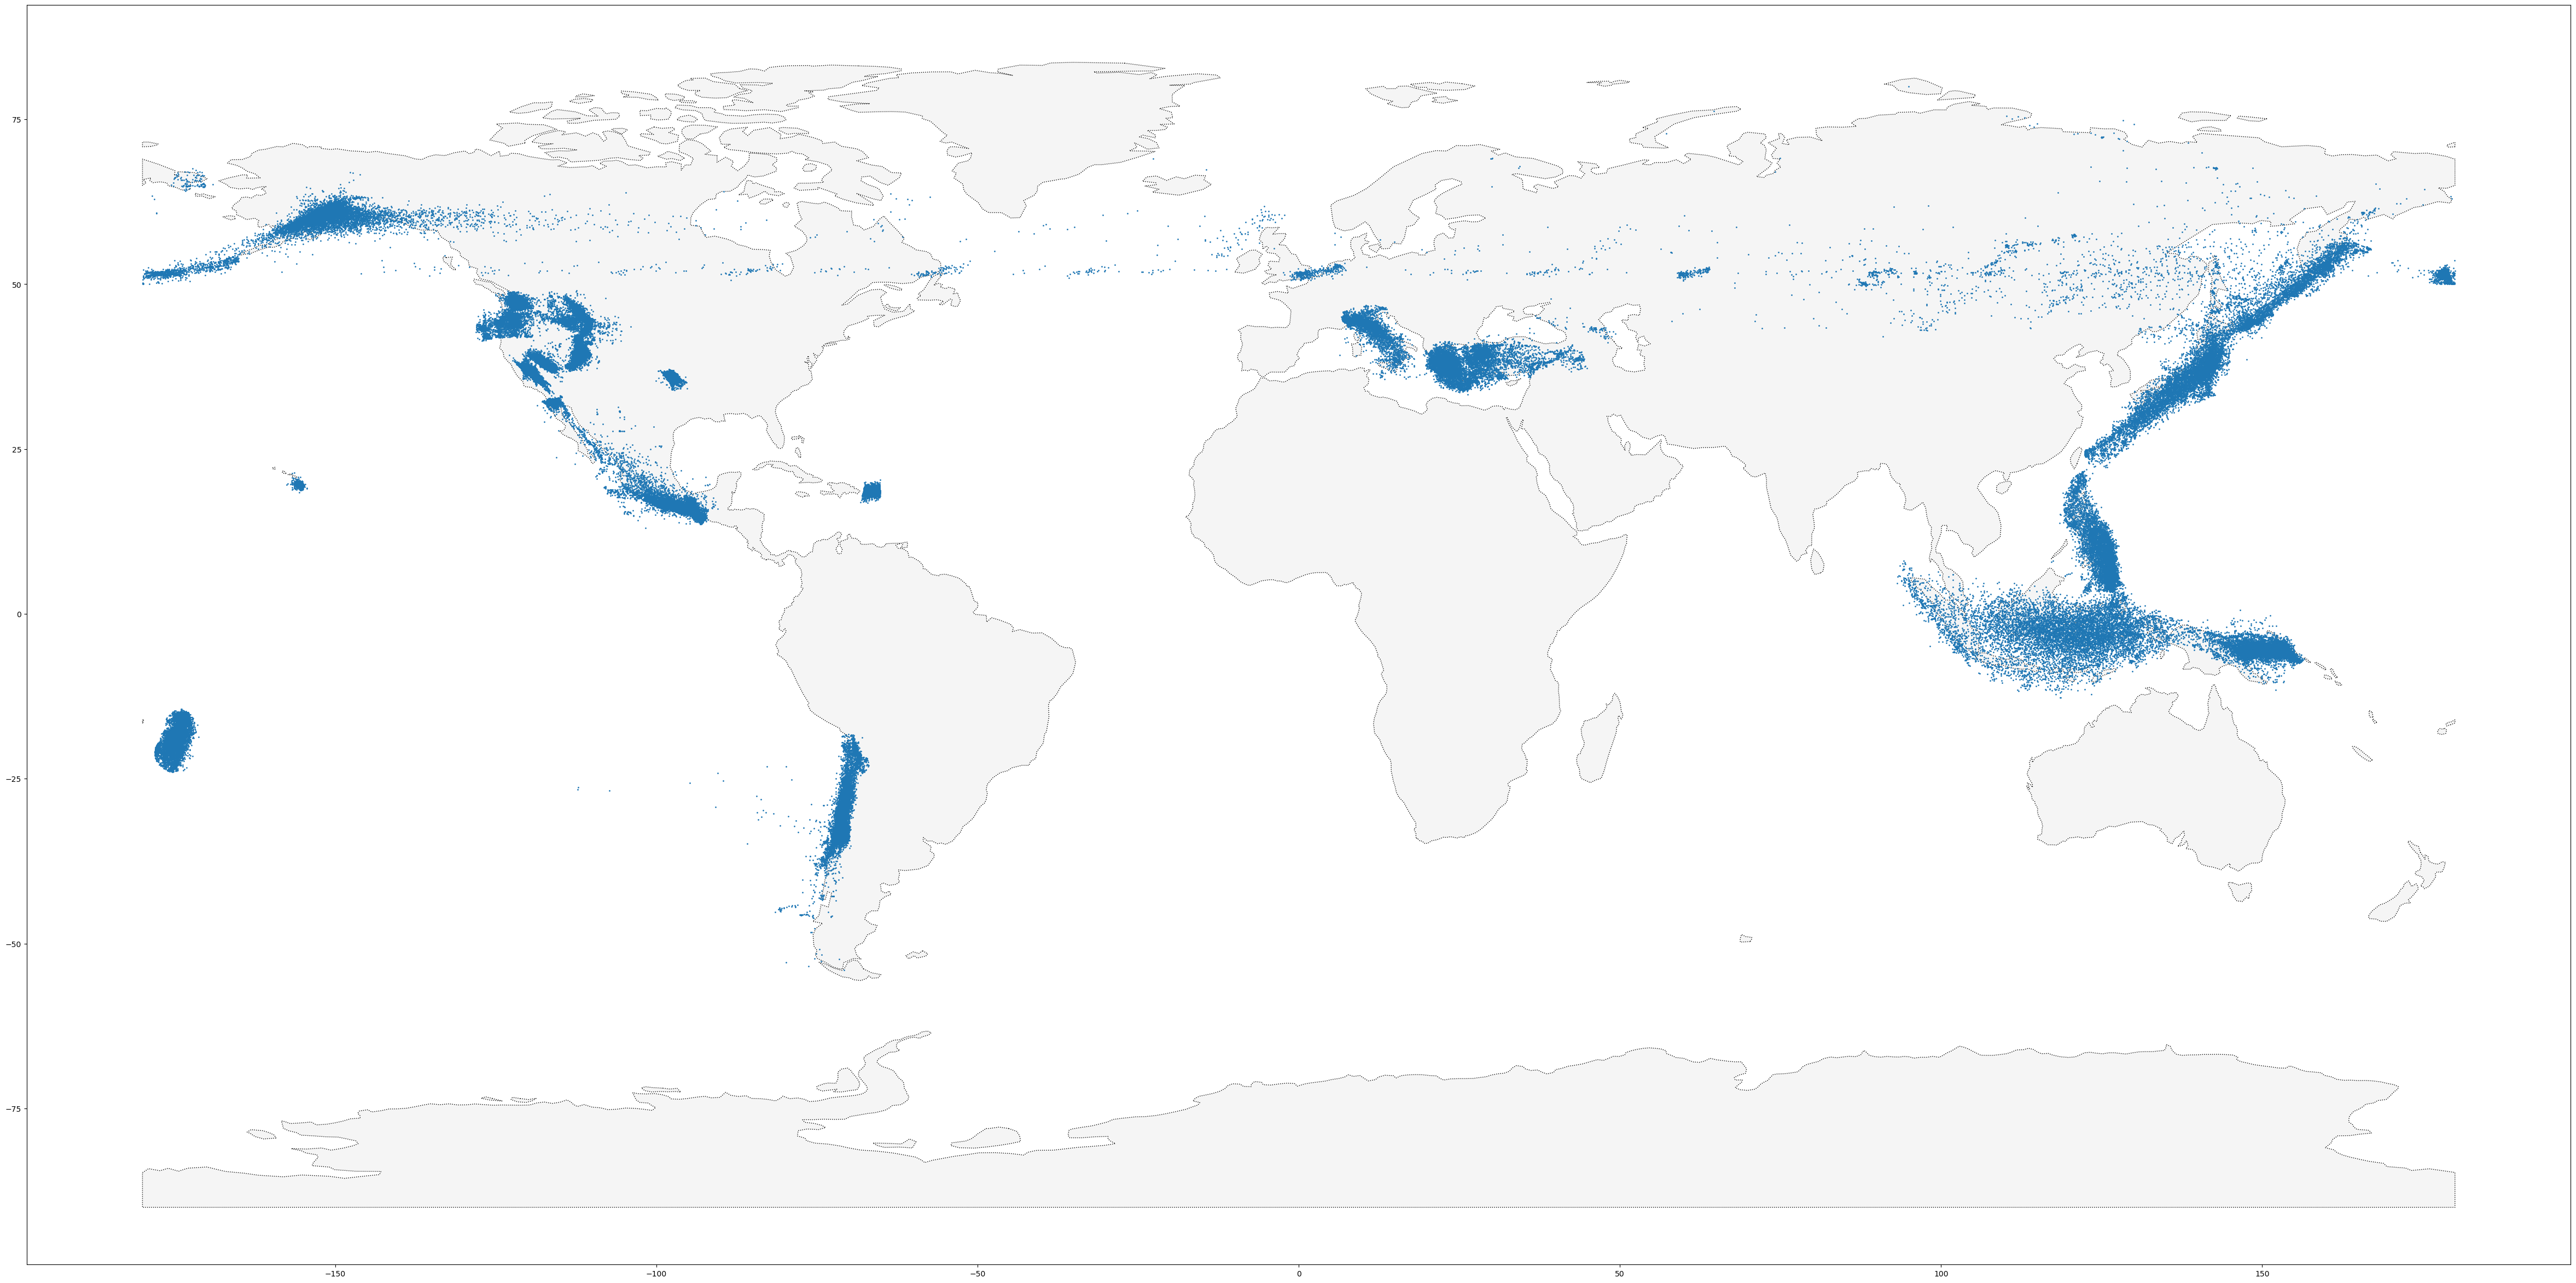
\includegraphics[scale=0.13]{img/world-earthquakes-top-25-regions-past-30-years.png}
  \captionsetup{format=hang}
  \caption{\label{fig:world-map}Top 25 regions with the highest number of earthquakes since 1974.}
\end{figure}

The dataset contained detailed information about the time, location (latitude and longitude),
depth, and magnitude of an occurring earthquake. Additionally, there are other features
available on the API. A detailed list can be found on the \ac{USGS} website
\footnote{\url{https://earthquake.usgs.gov/earthquakes/feed/v1.0/csv.php}}.

\subsubsection{Preprocessing}

Effective preprocessing is critical for handling the unique characteristics of
time series data, particularly in earthquake forecasting. In our study, we began
by addressing the unevenly spaced timestamps in the dataset. To standardize the
intervals, we opted for daily aggregation. While we also experimented with hourly
aggregation, it resulted in prohibitively long model training times - ranging
from 12 hours to a full day - making daily aggregation the more practical choice.

Our analysis revealed a strong time dependency for most values, extending up to
40 lags and potentially more in certain regions (Figure \ref{fig:pacf-sample};
\ref{fig:mag-acf-sample}; \ref{fig:depth-acf-sample}). This suggests that extensive
historical data would be beneficial for predictions. However, incorporating
such long historical windows significantly increases dimensionality, making
the model complex and computationally expensive. We question the practicality
of using nearly every recorded value in a region for forecasting future earthquake
occurrences, especially given that some regions have lags spanning multiple months or even years.
To address the dimensionality challenge, we capped the historical lags and the
exponential moving average at 7 days into the past. This compromise ensured that
we incorporated sufficient historical information while keeping the model
computationally feasible. Balancing the need for historical data without
overwhelming the model with too much information was crucial for our approach.

Our analysis of partial autocorrelation and autocorrelation functions
(Figure \ref{fig:pacf-sample};
\ref{fig:mag-acf-sample}; \ref{fig:depth-acf-sample}) revealed
that only the first few lags were significantly correlated in some regions.
This finding indicated that adding more lags beyond this point would not
improve predictive accuracy but would instead introduce unnecessary complexity.
Thus, capping historical lags at 7 days further validated our approach, focusing
model training on the most relevant temporal dependencies for effective earthquake
prediction in those specific regions.

\begin{figure}[hbtp]
  \centering
  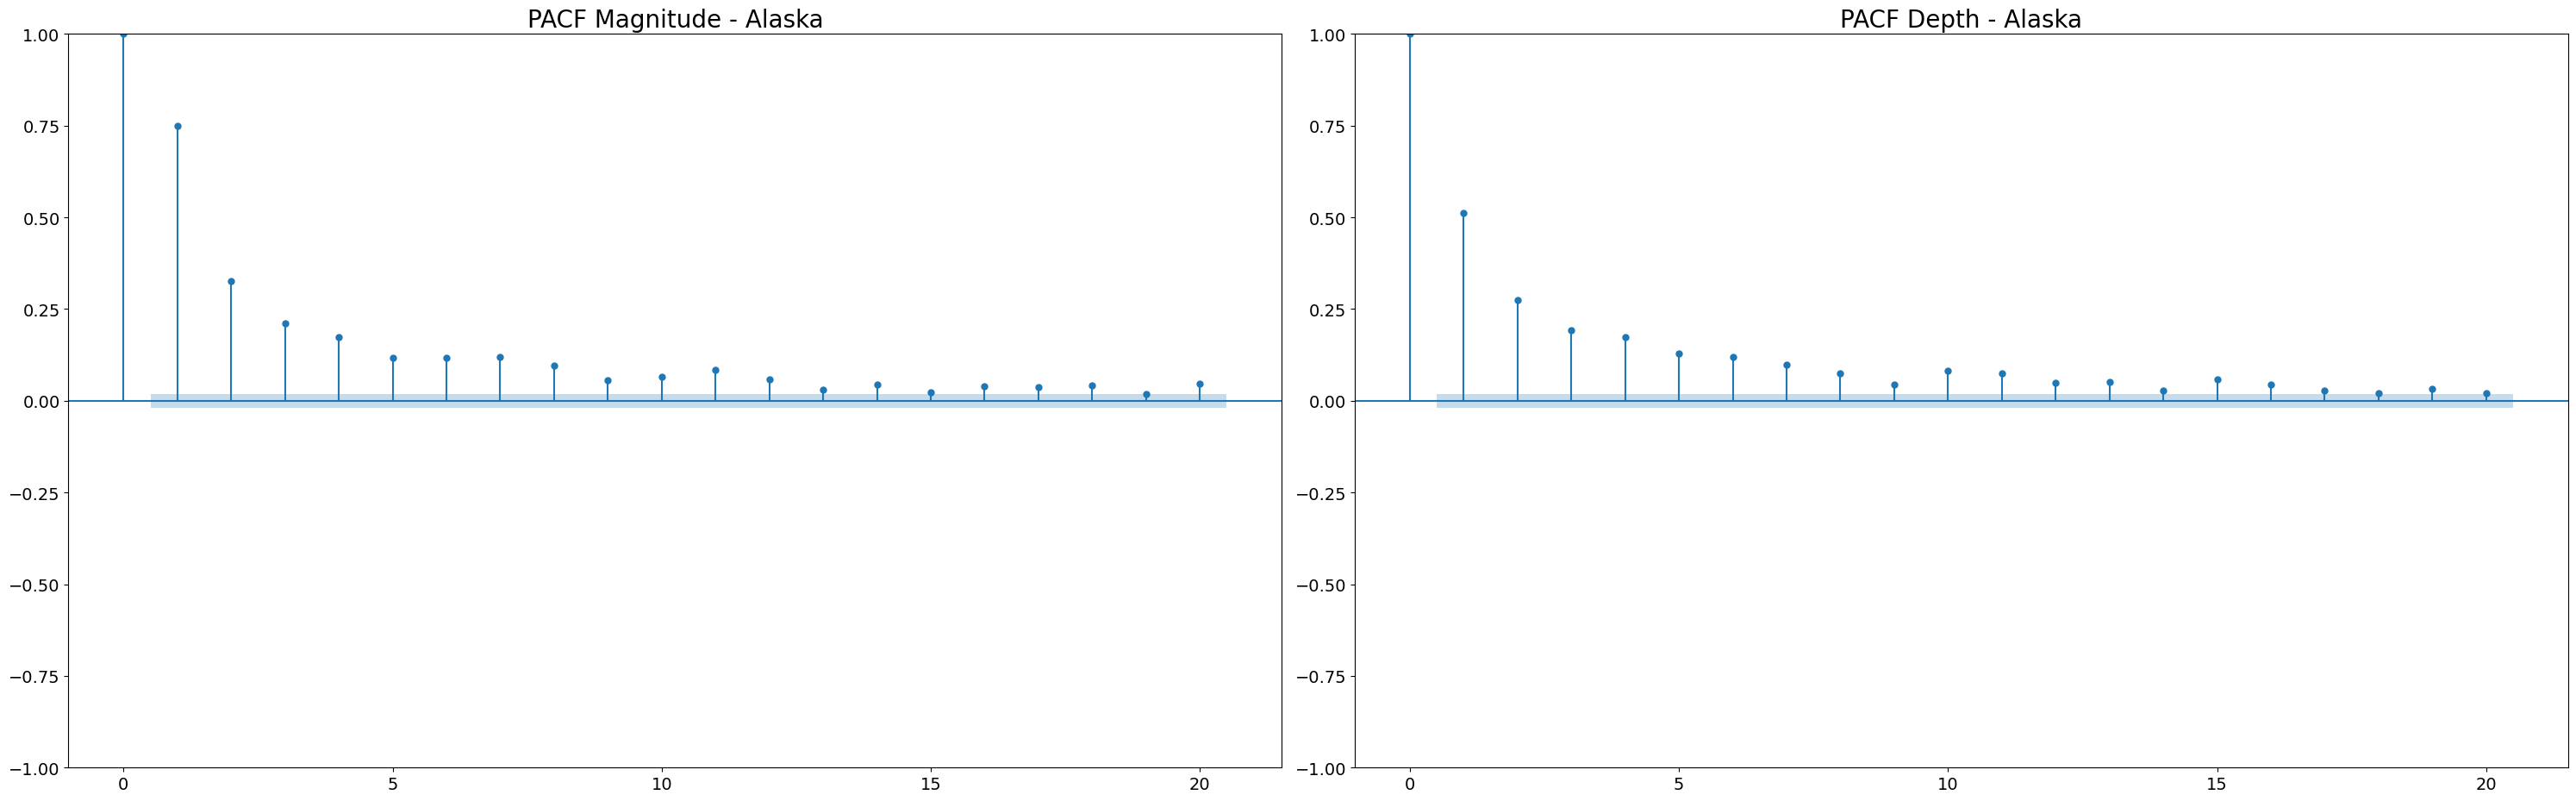
\includegraphics[scale=0.2]{img/pacf-sample.png}
  \captionsetup{format=hang}
  \caption{\label{fig:pacf-sample}Magnitude and depth partial autocorrelation of Alaska.
    The full details can be found in Appendix Figure \ref{fig:mag-pacf} (magnitude)
    and Figure \ref{fig:depth-pacf} (depth).}
\end{figure}

\begin{figure}[hbtp]
  \centering
  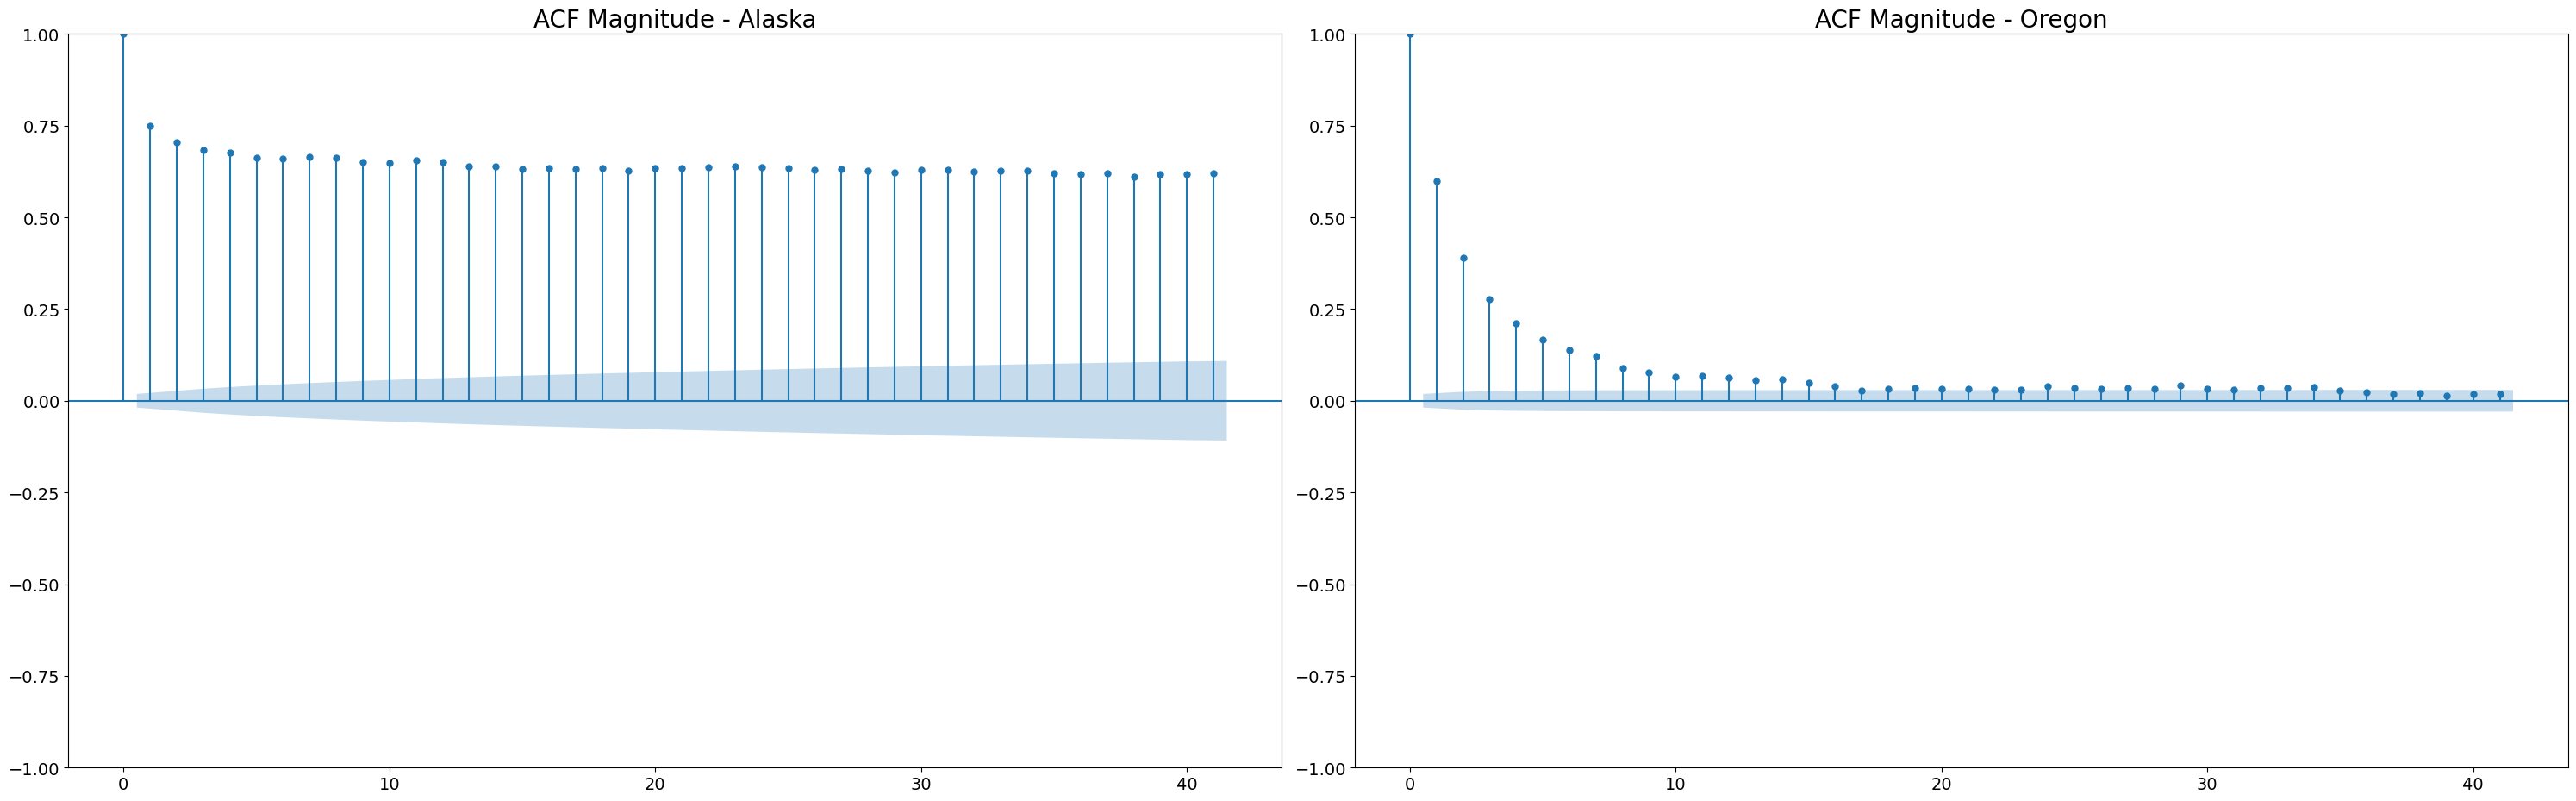
\includegraphics[scale=0.2]{img/magnitude-acf-sample.png}
  \captionsetup{format=hang}
  \caption{\label{fig:mag-acf-sample}Magnitude autocorrelation of Alaska and Oregon.
    The full details can be found in Appendix Figure \ref{fig:mag-acf}.}
\end{figure}

\begin{figure}[hbtp]
  \centering
  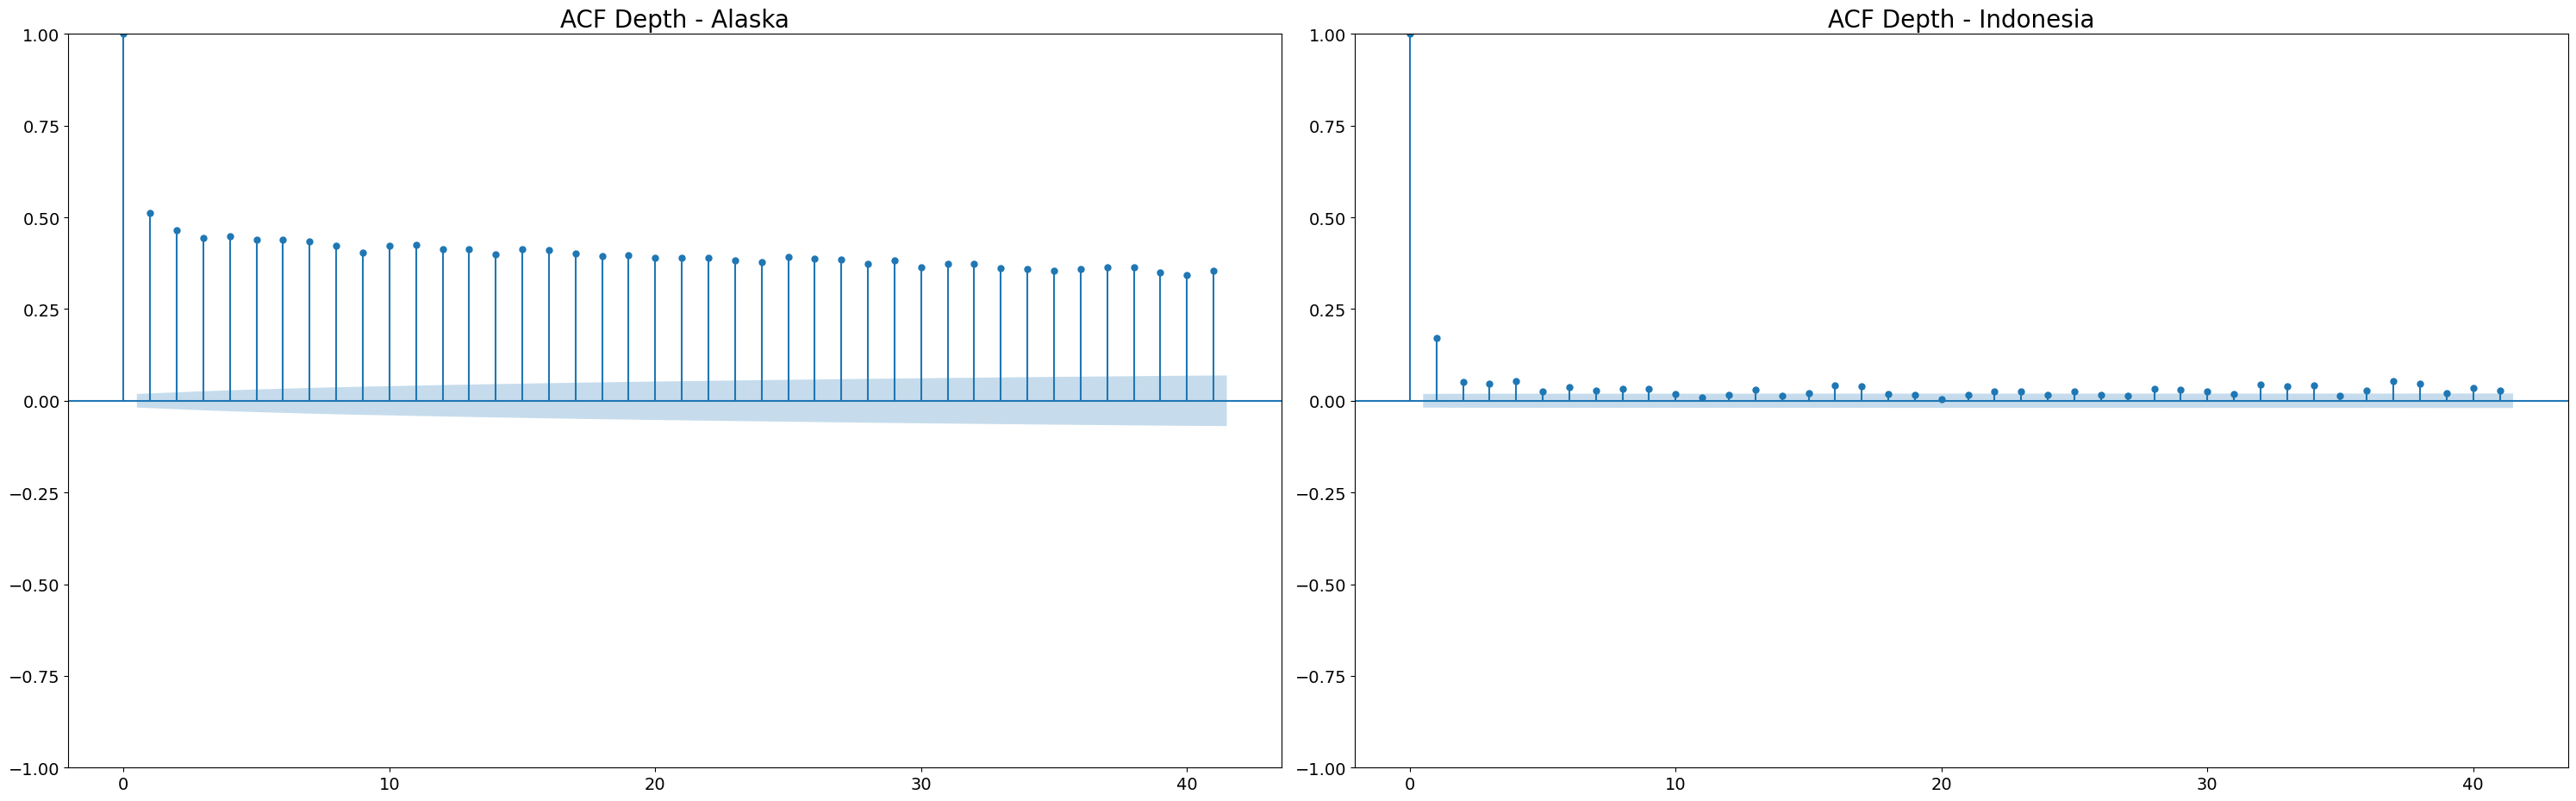
\includegraphics[scale=0.2]{img/depth-acf-sample.png}
  \captionsetup{format=hang}
  \caption{\label{fig:depth-acf-sample}Depth autocorrelation of Alaska and Indonesia.
    The full details can be found in Appendix Figure \ref{fig:depth-acf}.}
\end{figure}

Given that we are conducting global time series forecasting, these measures are
sufficient and appropriate. By capping the historical lags at 7 days, we successfully
balanced the need for historical information with the necessity of maintaining a
computationally feasible model. This strategy, backed by our autocorrelation analysis,
ensures that our model remains both efficient and accurate in predicting earthquake
occurrences on a global scale.

\begin{figure}[hbtp]
  \centering
  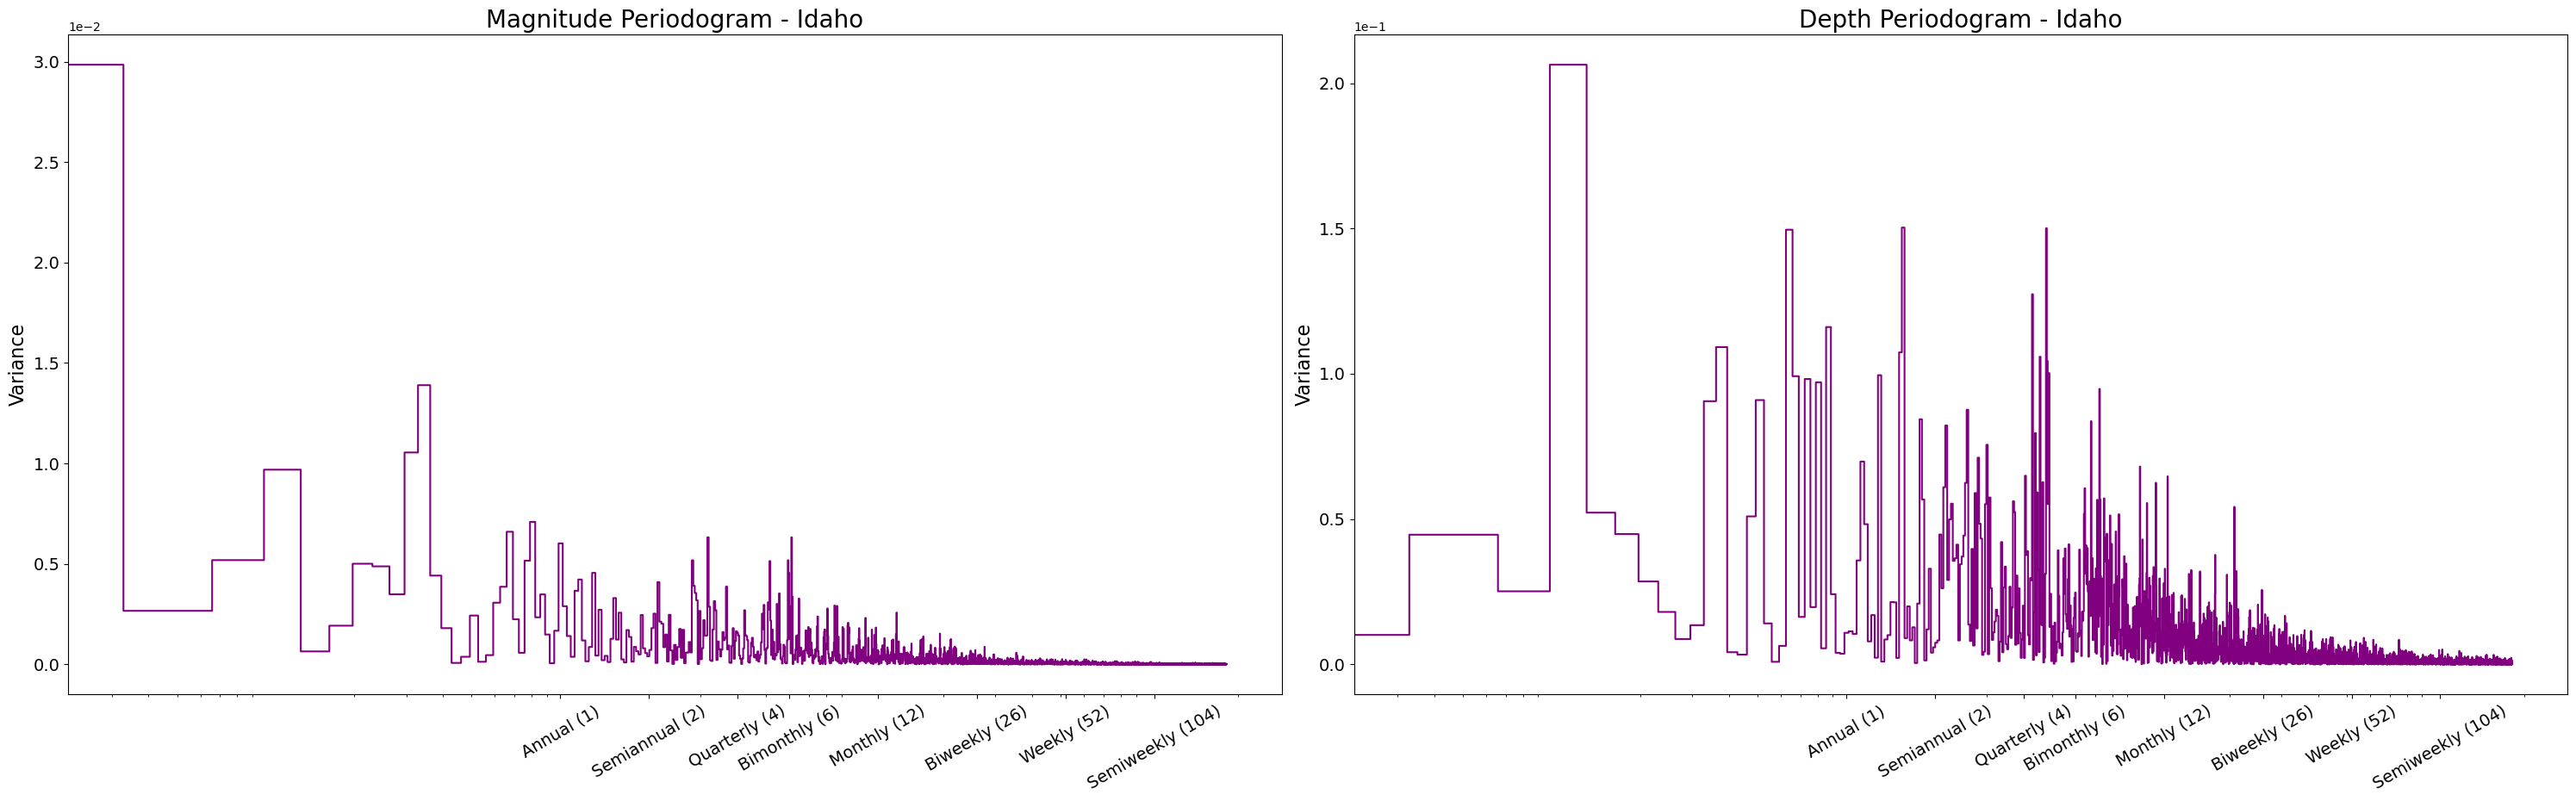
\includegraphics[scale=0.2]{img/periodogram-sample.png}
  \captionsetup{format=hang}
  \caption{\label{fig:periodogram-sample}Magnitude and depth periodogram of Idaho.
    The full details can be found in Appendix Figure \ref{fig:mag-periodogram} (magnitude)
    and Figure \ref{fig:depth-periodogram}.}
\end{figure}

Furthermore, our analysis of depth and magnitude periodograms (Figure \ref{fig:periodogram-sample})
indicated that earthquakes
exhibit a high degree of randomness, with some seasonality detected in only a minority
of regions. Due to this predominant randomness, using \ac{FFT}
to model seasonality proved impractical. Consequently, our preprocessing did not
rely on \ac{FFT}-based seasonal adjustments.

For model training, we implemented an 80-20 train-test split for each region. This
split was time-based, ensuring that past data was used to predict future values.
This method aligns with the temporal nature of the data and the forecasting goal,
allowing the model to learn from historical trends and apply this knowledge to
future predictions.

\subsection{Model}

To forecast earthquakes for 25 regions accurately, we employ a global forecasting model.
Among the various approaches available, tree-based models and \ac{RNNs}, specifically
\ac{LSTM} networks, are considered due to their ability to handle time-series data
effectively. For this particular application, we use CatBoost regression
\parencite{prokhorenkova2018catboost}, an efficient gradient boosting framework.

We chose CatBoost regression for forecasting earthquakes across 25 regions due to
its handling of categorical features, which simplifies preprocessing and ensures
robust feature encoding. CatBoost also offers better interpretability, allowing us
to understand the impact of different variables on predictions. Its training
efficiency and built-in mechanisms to prevent overfitting make it a practical
choice, particularly with the volatile nature of earthquake data. Additionally,
CatBoost can capture complex feature interactions without extensive feature
engineering, streamlining the modeling process and enhancing overall accuracy.

While tree-based models often struggle with forecasting trends, CatBoost regression
is particularly well-suited for our task for several reasons. The magnitude of
earthquakes is capped within a range of [-1, 10], and their depth falls within
  [-100, 1000] meters \parencite{earthquake-data}. In regression trees, predictions
are made by traversing a series of if-else conditions to reach a leaf node, where
the average of the values in that leaf are used for the prediction. Due to the
nature of these trees, it is not possible to predict values outside of those
observed in the training set. This makes CatBoost, with its advanced handling
of categorical features and robust performance on unseen data, an excellent
choice for this type of regression problem.

CatBoost transforms categorical features into numerical ones by employing
several methods, including random permutation of input objects and label
value conversion to integers, tailored to the type of machine learning problem
(regression, classification, or multi-classification). It calculates the
transformation using various statistics, such as counting occurrences within
specific buckets or calculating mean target values. The primary formula for
this transformation is:

\[\text{ctr} = \frac{\text{countInClass} + \text{prior}}{\text{totalCount} + 1}\]

where \textit{countInClass} is the relevant label count, \textit{prior} is a
predefined constant, and \textit{totalCount} is the cumulative count of objects
with the same categorical value. Additionally, CatBoost supports one-hot encoding
for categorical features with limited unique values, controlled by the
\textit{one\_hot\_max\_size} parameter \parencite{catboost-encoding}.

To forecast earthquakes, we predict magnitudes and depths, while for location
(latitude and longitude), we compute the historic median to reduce model
complexity and enhance stability. The forecasting process is performed
recursively or iteratively: initially, we forecast the data for one day,
using the predicted values to create features for the subsequent day.
This process is repeated, building on each previous prediction, until
forecasts for three days are generated. This recursive approach allows
the model to adapt dynamically to the changing conditions and trends
observed in the time series data, providing more accurate and reliable forecasts.

\subsubsection{Training}
The model training process for earthquake forecasting requires a structured
approach, beginning with a careful feature selection. The chosen features
include temporal attributes such as the day, day of the week, and day of
the year, which capture the time-dependent aspects of earthquake occurrences.
Additionally, exponential moving averages for both magnitude and depth are
included to reflect the trends over recent periods. The model also incorporates
lagged values for magnitude and depth over a specified range, allowing it to
consider past events' influence on current conditions. The inclusion of the
categorical feature region ensures that the model can account for regional
differences in earthquake behavior.

The chosen model for this task is the CatBoost Regressor, selected for its
ability to handle categorical features natively and its strong performance
with complex datasets. The model is configured with early stopping rounds to
mitigate overfitting and is optimized using the MultiRMSE loss function, which
targets minimizing errors in both magnitude and depth predictions. The training
dataset comprises the selected features and the categorical region feature,
while the target variables are the earthquake magnitude and depth.

To enhance the model's performance, hyperparameter tuning is performed using
grid search, as shown in Table \ref{table:hyperparameters}. This involves
testing various combinations of hyperparameters
such as learning rate, model depth, and L2 leaf regularization. The grid
search evaluates these combinations to identify the optimal parameters that
yield the best predictive performance. This systematic approach to feature
selection, data preparation, and hyperparameter tuning aims to develop a
robust and accurate model capable of forecasting earthquake magnitude and
depth across different regions.

\begin{table}[h!]
  \centering
  \begin{tabular}{ll}
    \toprule
    \textbf{Hyperparameter} & \textbf{Values}          \\ \midrule
    Learning Rate           & 0.01, 0.03, \textbf{0.1} \\ \midrule
    Depth                   & 4, 6, \textbf{10}        \\ \midrule
    L2 Leaf Regularization  & 1, 3, \textbf{5}, 7, 9   \\ \bottomrule
  \end{tabular}
  \caption{Hyperparameter values explored during grid search. Best hyperparameters highlighted in bold.}
  \label{table:hyperparameters}
\end{table}

\subsubsection{Evaluation}
After training the CatBoost Regressor model for earthquake forecasting,
it is crucial to evaluate its performance using several metrics and visualization techniques.
The performance of the time series forecasting model is assessed using a variety of
metrics that provide a comprehensive view of its accuracy and reliability. The selected
metrics are the \ac{MAE}, the \ac{RMSE}, the R2-Score and the adjusted R2 Score
(Table \ref{table:model-metrics}).
These metrics collectively offer insights into the error magnitude and the goodness-of-fit
of the model. The rationale behind these metrics is explained in \ref{sec:Forecasting}.

\begin{table}[H]
  \centering
  \begin{tabular}{ll}
    \toprule
    \textbf{Metric} & \textbf{Score} \\ \midrule
    MAE             & 2.9344         \\ \midrule
    RMSE            & 10.3577        \\ \midrule
    R2              & 0.9495         \\ \midrule
    Adjusted R2     & 0.9495         \\ \bottomrule
  \end{tabular}
  \caption{Model metrics.}
  \label{table:model-metrics}
\end{table}

For our model, the MAE is 2.9344 (Figure \ref{table:model-metrics}), indicating
that on average, the predictions are approximately 2.9344 units away from the
actual values. Lower MAE values suggest better predictive accuracy, and the
obtained MAE value demonstrates that the model has a reasonably low level of error.

The RMSE for our model is 10.3577 (Figure \ref{table:model-metrics}),
which reflects the model's error magnitude.
While RMSE values are generally higher than MAE due to the squaring of errors,
they provide an important perspective on how significant the larger errors are
in the context of the model's predictions. A lower RMSE indicates a better fit,
and our RMSE value suggests a reasonable performance with some sensitivity to larger errors.

For our model, the R2 is 0.9495 (Figure \ref{table:model-metrics}), signifying
that approximately 94.95\% of the variance in the data is explained by the model.
This high R2 value suggests that the model fits the data very well and is capable
of capturing the underlying patterns in the time series.

The Adjusted R2 for our model is 0.9495 (Figure \ref{table:model-metrics}),
which is very close to the R2 value. This indicates that the inclusion of
predictors in the model is justified and that the model does not overfit the data.
The slight difference between R2 and Adjusted R2 confirms that the model maintains
a high level of explanatory power while accounting for the number of predictors.

The evaluation of the model using these metrics provides a well-rounded
understanding of its performance. The low MAE and RMSE values indicate
that the model has a low level of error, while the high R2 and Adjusted
R2 values demonstrate a strong fit to the data. Together, these metrics
suggest that the model is both accurate and reliable for forecasting the
time series data, making it a valuable tool for predicting future values.

In Appendix Figure \ref{fig:mag-forecast-full}, the magnitude forecasts demonstrate
varying degrees of accuracy across the different regions. For regions
like Alaska and Nevada, the model's predictions closely follow the
actual magnitudes, indicating a high level of accuracy. However, in
regions such as Indonesia and Chile, there are noticeable deviations
between the forecasted and actual values, suggesting areas where the
model could be improved. Overall, while the model captures the general
trends and fluctuations in earthquake magnitudes reasonably well, the
precision varies significantly by region. A sample of magnitude forecasts
is illustrated in Figure \ref{fig:mag-forecast}.

\begin{figure}[hbtp]
  \centering
  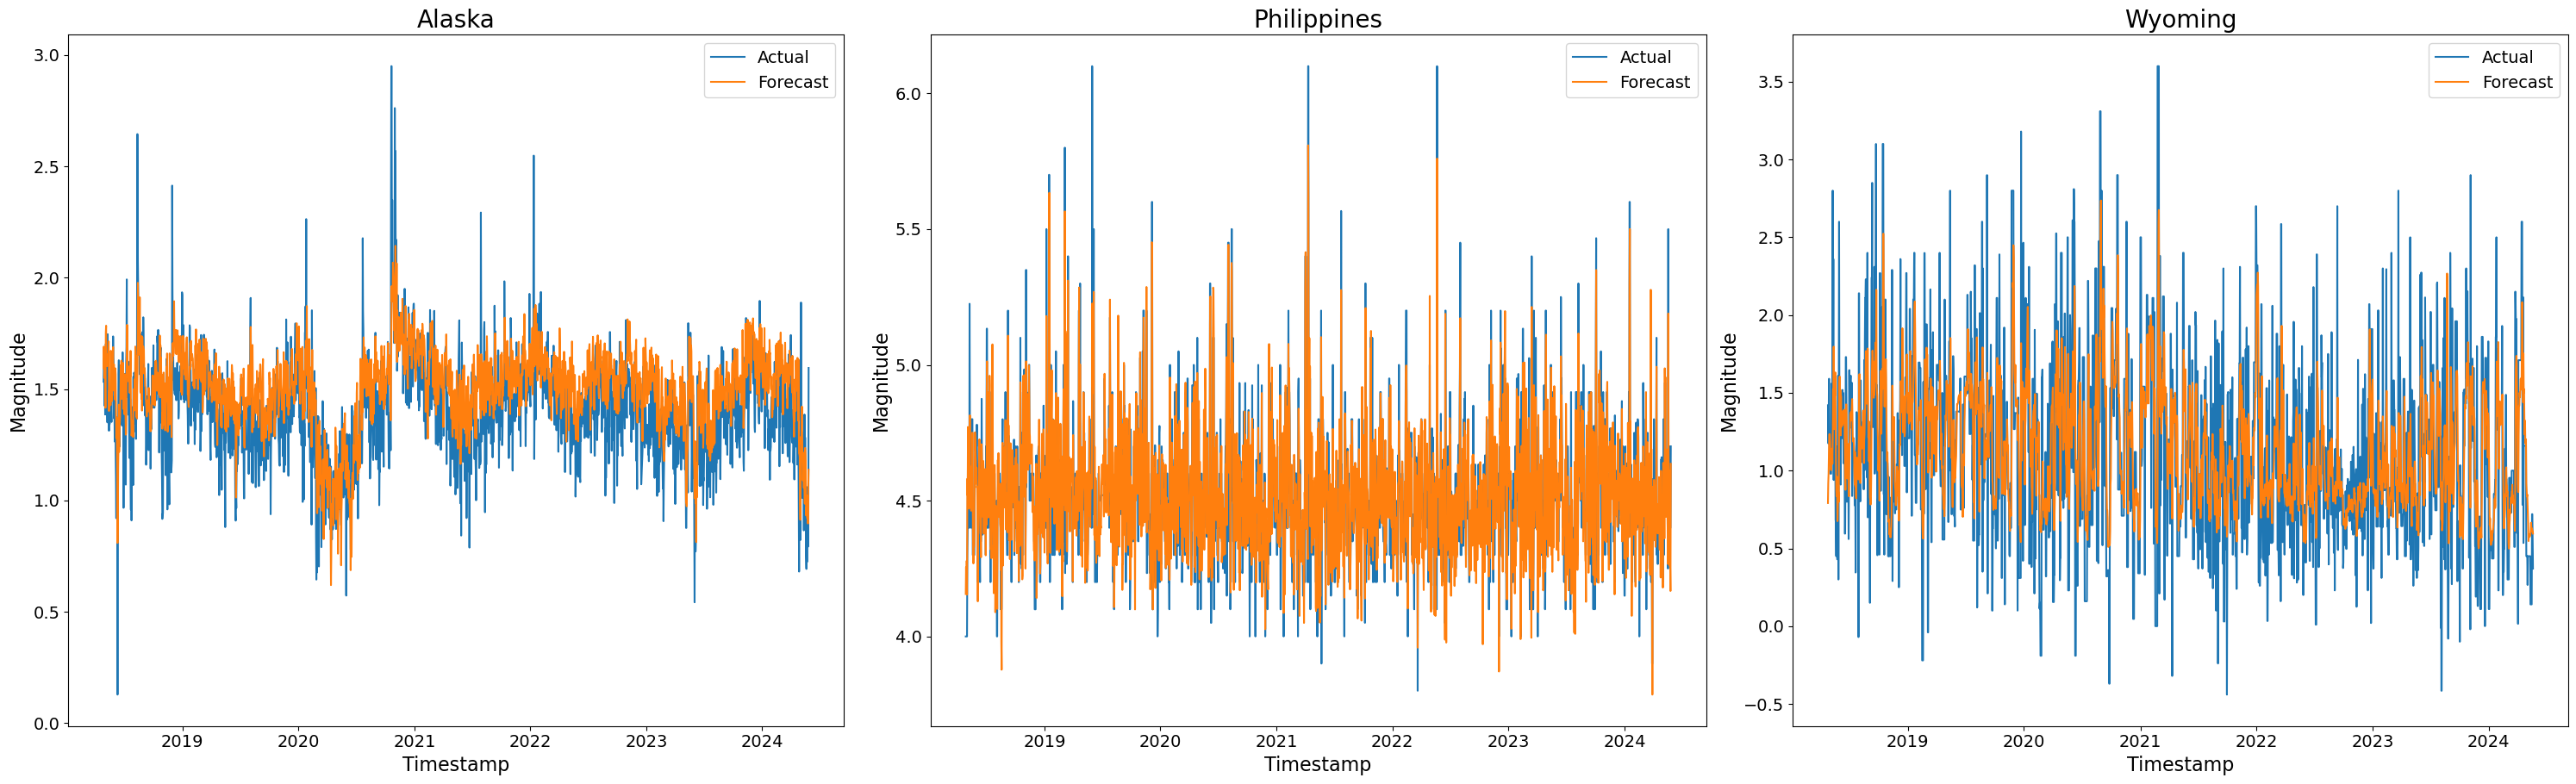
\includegraphics[scale=0.2]{img/magnitude-forecast-sample.png}
  \captionsetup{format=hang}
  \caption{\label{fig:mag-forecast}Magnitude forecast sample of Alaska (solid performance),
    Philippines (good performance), and Wyoming (suboptimal performance).}
\end{figure}

Appendix Figure \ref{fig:depth-forecast-full} focuses on the depth forecasts.
Similar to the magnitude forecasts, the depth predictions show
regional variability in accuracy. In regions such as Alaska,
California, and Nevada, the forecasted depths align closely
with the actual depths, indicating strong predictive performance.
Conversely, in regions like Indonesia and Papua New Guinea, the
forecasted depths show more significant discrepancies from the
actual values, highlighting potential areas for model enhancement.
A sample of depth forecasts is illustrated in Figure \ref{fig:depth-forecast}.

\begin{figure}[hbtp]
  \centering
  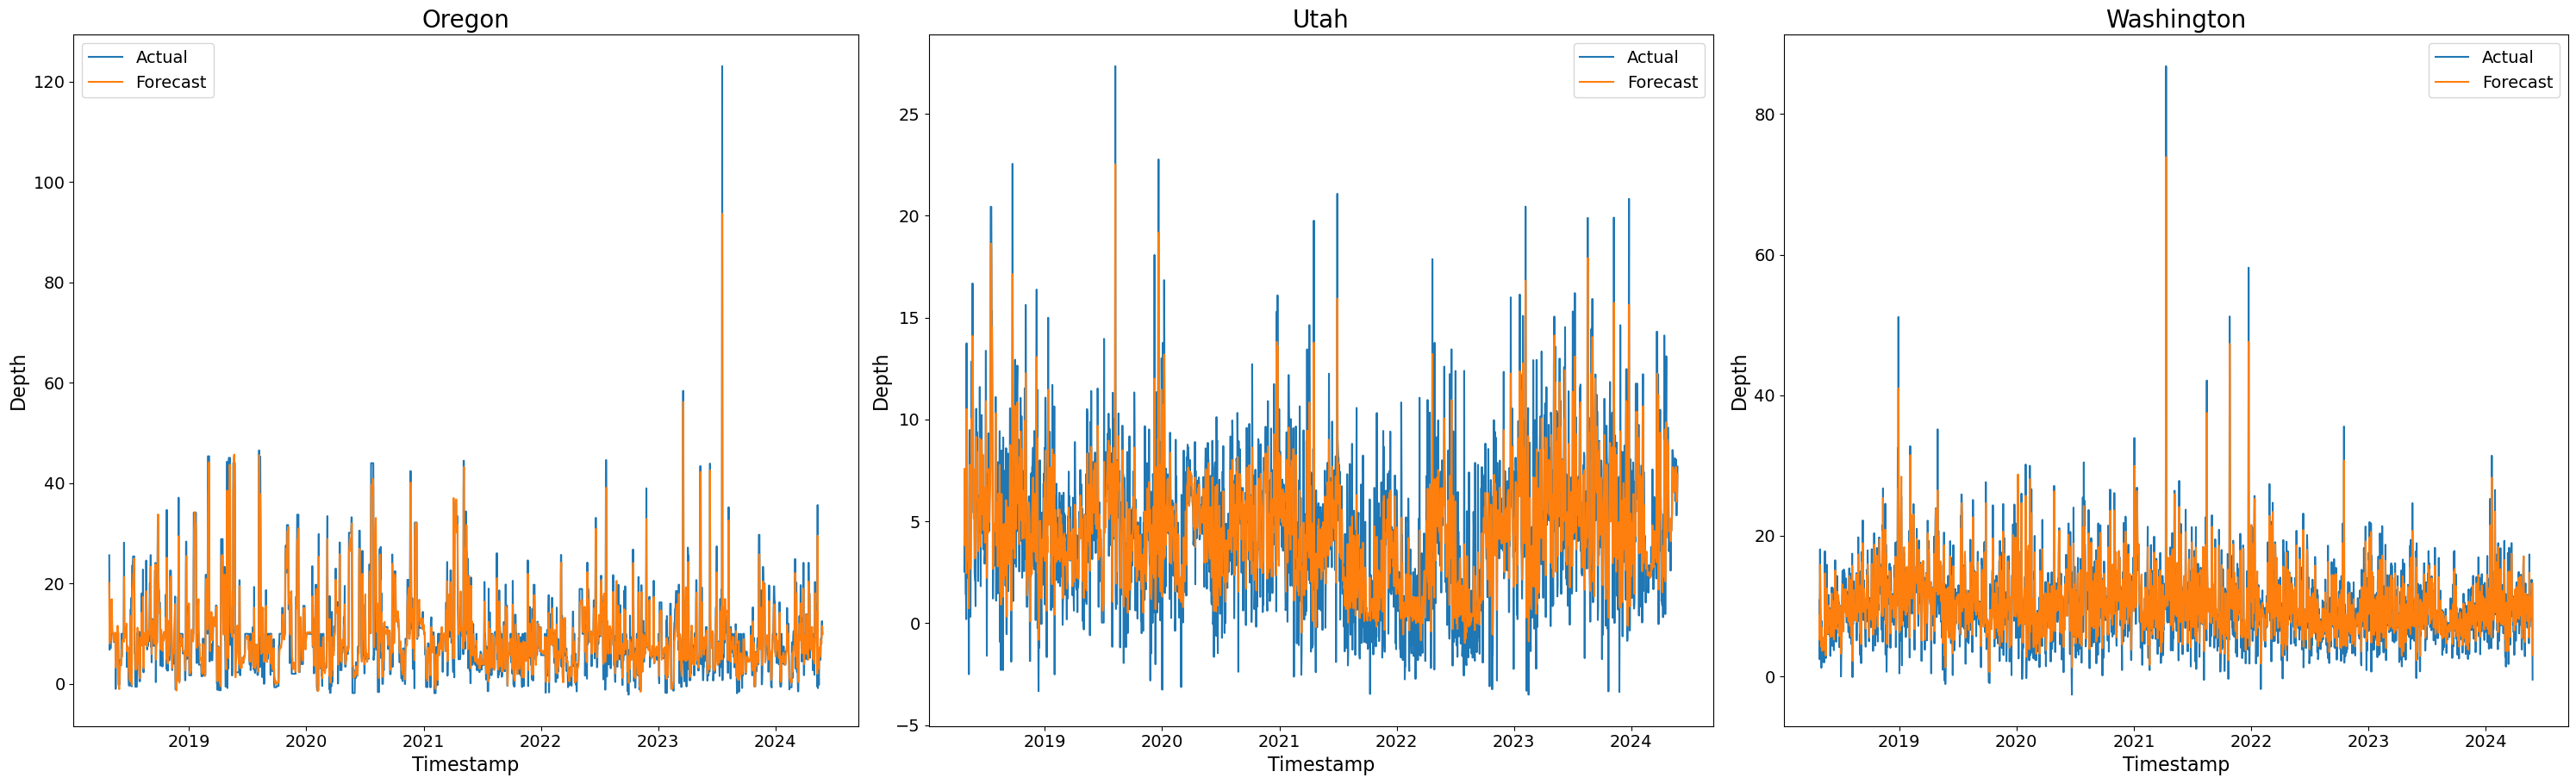
\includegraphics[scale=0.2]{img/depth-forecast-sample.png}
  \captionsetup{format=hang}
  \caption{\label{fig:depth-forecast}Depth forecast sample of Oregon (good performance),
    Utah (suboptimal performance), and Washington (solid performance).}
\end{figure}

Combining the insights from both sets of forecasts, it is evident
that the model's performance is influenced by regional characteristics.
The regions with higher accuracy in both magnitude and depth forecasts,
such as Alaska and Nevada, suggest that the model effectively captures
the underlying patterns in these areas. In contrast, regions with lower
accuracy, such as Indonesia and Chile, may require additional data or
model adjustments to improve predictive performance. Overall, the
model demonstrates a better capability for forecasting future depths than magnitudes.

While the model's evaluation metrics, including \ac{MAE}, \ac{RMSE}, R2, and Adjusted R2,
indicate excellent performance in terms of accuracy and goodness-of-fit,
it is important to acknowledge a significant limitation: the inherent
unpredictability of earthquakes. Earthquakes are fundamentally random
events, much like predicting stock market values, making them
exceptionally challenging to forecast with high precision. Despite
the model's robust statistical indicators, the chaotic and complex
nature of seismic activities means that accurate prediction remains
elusive. Thus, while the model shows promising results according to
the chosen metrics, its practical applicability in earthquake
forecasting is constrained by the unpredictable and stochastic
nature of the phenomenon itself.

\begin{figure}[hbtp]
  \centering
  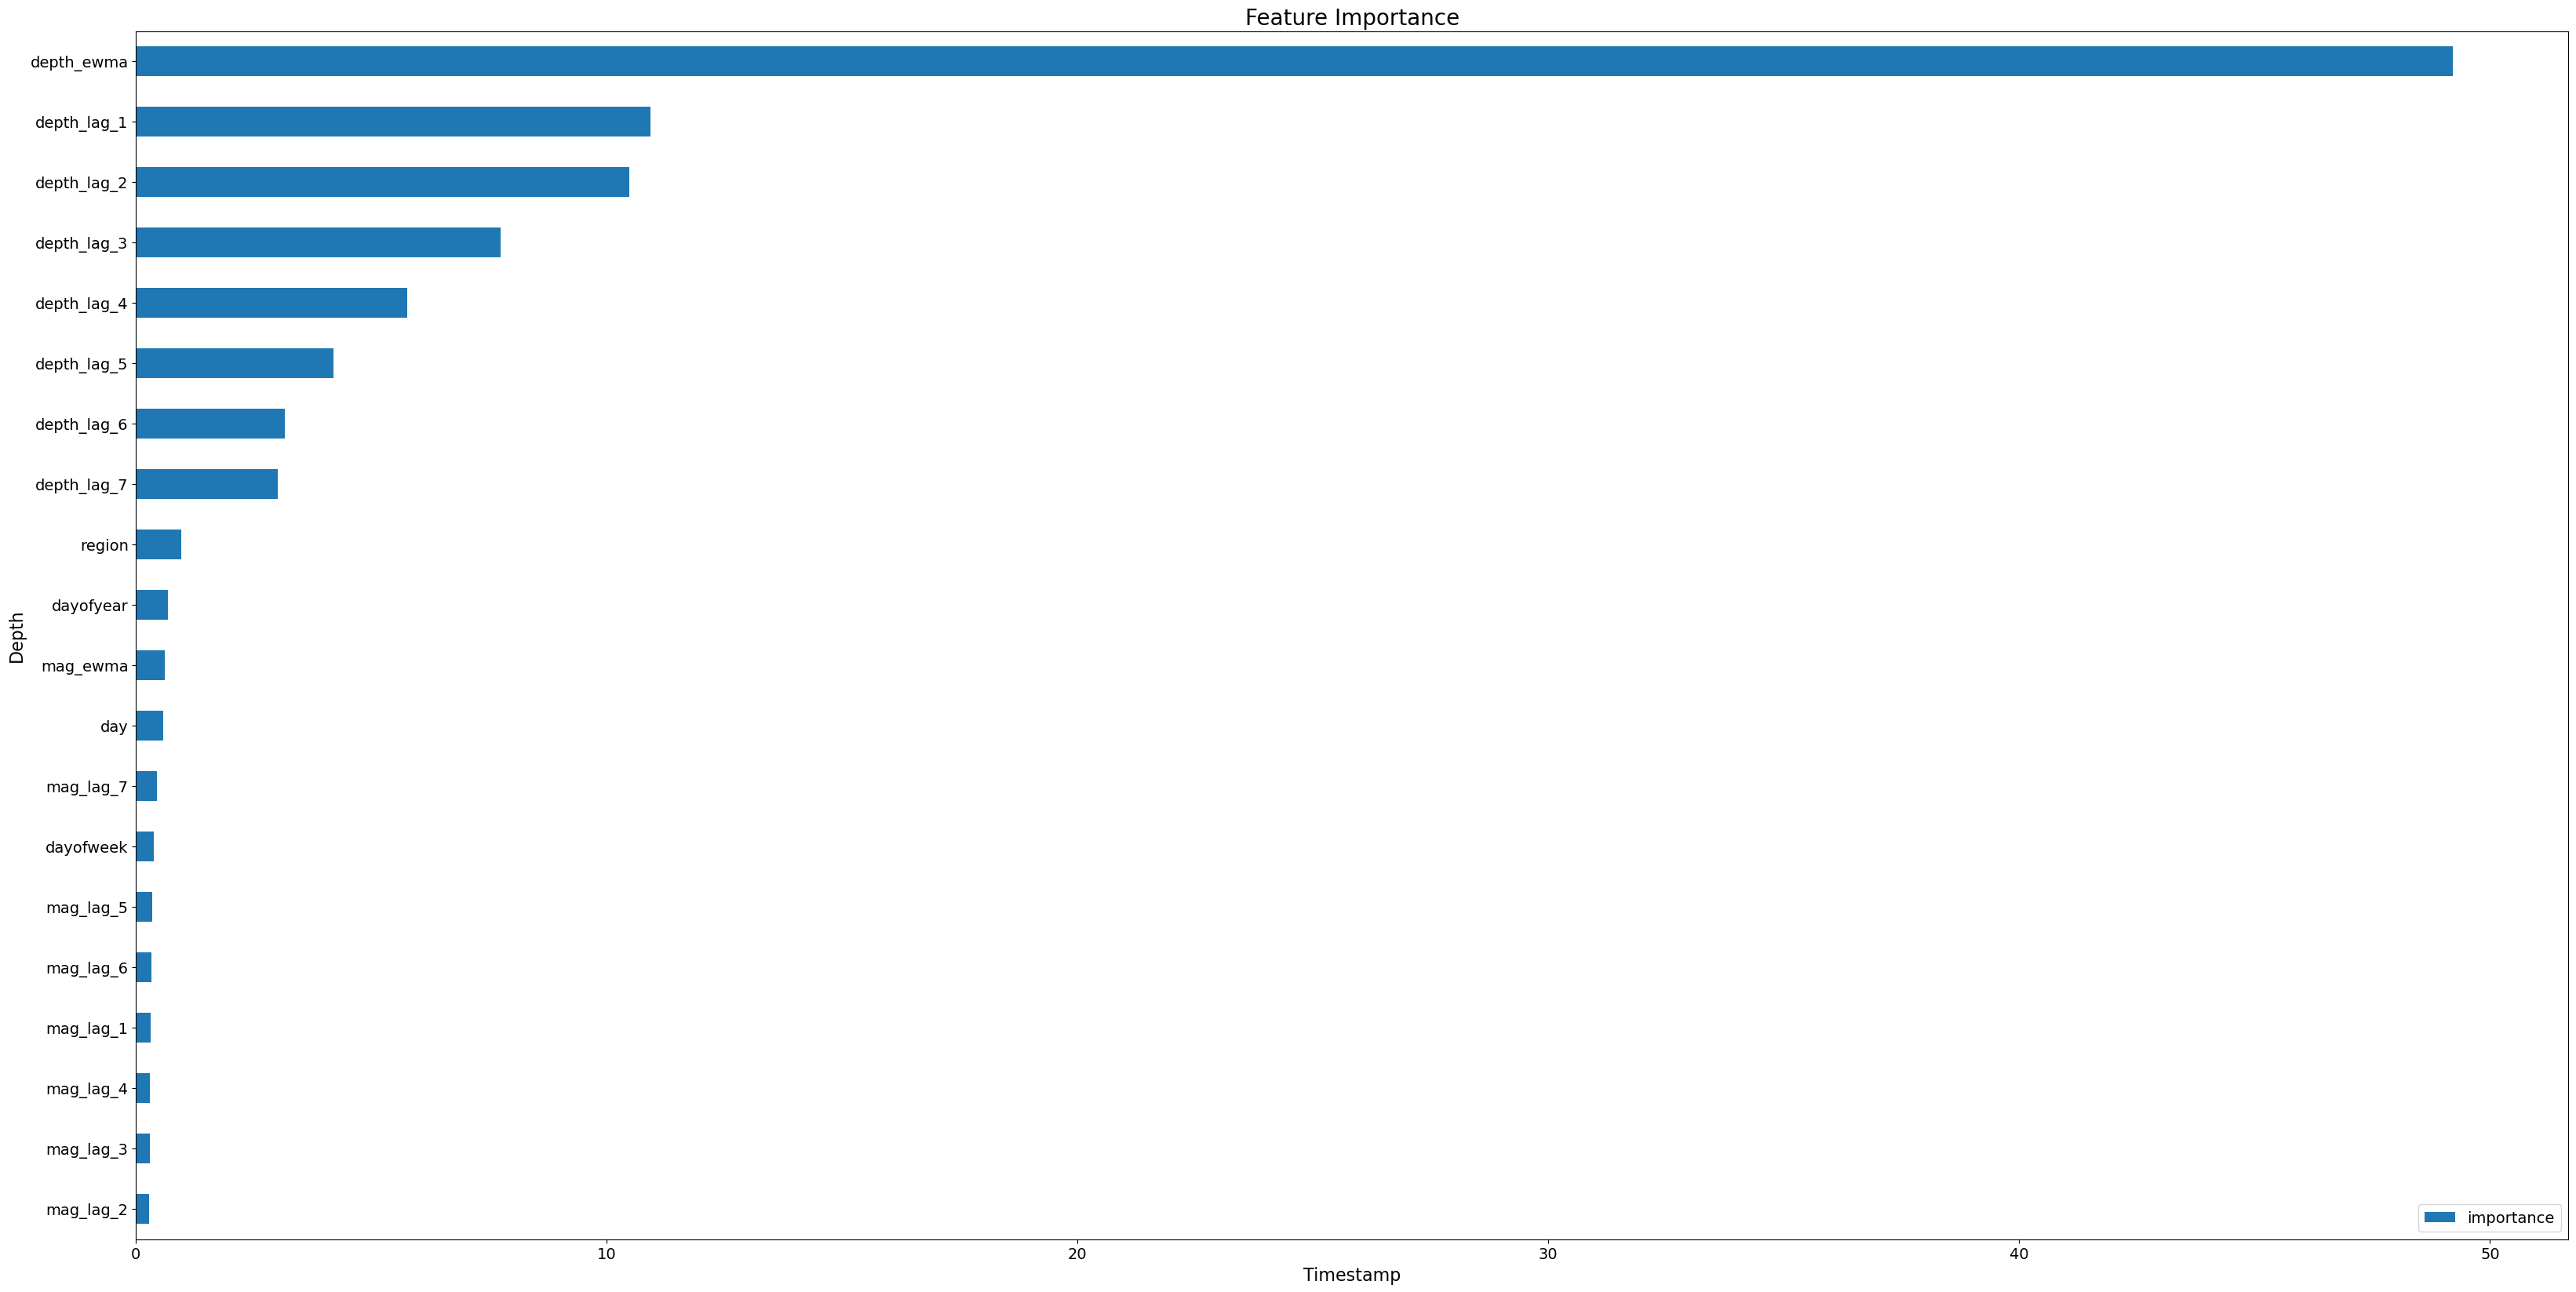
\includegraphics[scale=0.18]{img/model-feature-importance.png}
  \captionsetup{format=hang}
  \caption{\label{fig:feature-importance}Feature importance}
\end{figure}

The feature importance plot displayed in Figure \ref{fig:feature-importance}
highlights the significance of various input features in a forecast model that
predicts the magnitude and depth of earthquakes. Notably, the feature
\textit{depth\_ewma} (exponential moving average of depth) stands out as
the most critical feature by a considerable margin, indicating its paramount
influence on the model's predictions. Following \textit{depth\_ewma},
features such as \textit{depth\_lag\_1}, \textit{depth\_lag\_2}, and
\textit{depth\_lag\_3} also demonstrate significant importance, suggesting
that recent depth values have a substantial impact on the forecast. In
contrast, features related to the earthquake magnitude, such as
\textit{mag\_ewma} (exponential moving average of magnitude) and various
magnitude lags, show much lower importance, indicating a lesser role in
the prediction model. Additionally, temporal features like \textit{dayofyear}
and \textit{dayofweek} have minimal impact. This analysis underscores that
the recent history of earthquake depth, especially its exponential moving
average, is the most influential factor in forecasting future earthquake
magnitudes and depths.

\section{LLM-powered AI Agent}
Advancements in AI have given rise to AI agents as powerful tools
for enhancing productivity and communication \parencite{xi2023rise}.
Equipped with \ac{LLM}s, these agents can perform a wide array of tasks,
such as information processing, creative text generation, language
translation, and providing insightful responses to inquiries.

Unlike conventional virtual assistants and chatbots, AI agents operate
based on learned patterns and data, enabling them to offer more nuanced
understanding and communication. For instance, an AI agent trained on
extensive datasets of text and code can retrieve pertinent articles,
distill key findings into summaries, or craft tailored content based
on the preferences of specific target audiences. The potential
applications of LLM-powered AI agents are vast and diverse, ranging
from automating repetitive tasks to supporting complex decision-making
processes and creative endeavors. However, it is crucial to recognize
that while AI agents excel in language manipulation and generation, they
lack true sentience or consciousness, necessitating responsible usage to
mitigate the risk of biased or misleading content generation.

\subsection{Instructions}

The AI agent uses a combination of tools to deliver accurate and timely
earthquake forecasts. The agent is built using the ReAct prompting
\parencite{yao2023reactsynergizingreasoningacting} method as shown in
Source Code \ref{lst:system-prompt}, which enhances its interaction
capabilities and allows it to provide expert-level responses regarding earthquakes.
An example of the LLM-powered AI agent in action can be found in Appendix Figure
\ref{fig:copilot}.

\begin{lstlisting}[caption={\texttt{system\_prompt.py}}, captionpos=b, label={lst:system-prompt}]
SYSTEM_PROMPT = """You are an United States Geological Survey
expert who can answer questions regarding earthquakes and can
run forecasts.

Before you use the Forecast Earthquakes tool, always check
which regions are available using Find Regions first.
Respond to the user as helpfully and accurately as possible.

You have access to the following tools:
{tools}

Please ALWAYS use the following JSON format:
{{
  "thought": "Explain your thought. Consider previous and
    subsequent steps",
  "tool": "The tool to use. Must be on of {tool_names}",
  "tool_input": "Valid keyword arguments (e.g. {{"key": value}})",
}}

Observation: tool result
... (this Thought/Tool/Tool input/Observation can repeat N times)

When you know the answer, you MUST use the following JSON format:
{{
  "thought": "Explain the reason of your final answer
    when you know what to respond",
  "tool": "Final Answer",
  "tool_input": "Valid keyword arguments (e.g. {{"key": value}})",
}}"""
\end{lstlisting}

ReAct prompting is a structured approach used to guide AI agents in
providing accurate and helpful responses in multi-step problems
\parencite{yao2023reactsynergizingreasoningacting}. The agent is
programmed with a specific system prompt that positions it as a
United States Geological Survey (USGS) expert. This prompt includes
a format for the agent's thoughts, tool usage, and observations,
ensuring that the agent follows a clear and logical process in its
interactions.

Even though we define a specific output format, the LLM still predicts
the most likely token that should come next, which can lead to errors
in the output format, such as responding with text instead of JSON.
This process can be compared to a trial-and-error learning process.
We then enter a loop of refinement. If the LLM's output can't be
parsed into the correct format, it's reminded of the requirement
and prompted to adjust. Conversely, a successful parse leads to the
LLM's output being used to call a relevant tool. If the tool call
fails, the LLM is asked to refine it further. This cycle continues
until a satisfactory answer is produced, either through a parsable
output or the LLM exhausting its attempts. This iterative process
ensures continuous feedback and correction, ultimately aiming to
achieve the desired outcome: a correct response in the specified format.

Explainable AI agents play a crucial role in fostering trust and
transparency with users by allowing them to understand the
decision-making processes of \ac{LLM}s. Through the use of
techniques such as ReAct prompting \parencite{yao2023reactsynergizingreasoningacting},
we can visibly demonstrate what the LLM is doing behind the scenes. This
involves showing the sequence of actions taken by the model, including
its thoughts, the tools employed, the input provided to these tools,
the tools' responses, and the model's subsequent thoughts leading to
the final answer. By offering this level of insight, we can build
greater confidence in the LLM's outputs and facilitate a more
informed interaction with the technology. An example is shown in Appendix Figure
\ref{fig:explainable-ai}.

\subsection{Tools}

The AI agent designed for earthquake forecasting integrates several tools
to provide accurate and comprehensive information. These tools, leveraging
forecasting models and data processing techniques, enhance the agent's
capability to predict and analyze seismic events. Here’s a detailed
look at the tools used by the AI agent:

\begin{enumerate}
  \item \textbf{Current Date:} This tool provides the current
        local date and time. It is essential for timestamping queries
        and ensuring that all data processing is aligned with the
        date the user asked about.
  \item \textbf{Query Earthquakes:} This tool searches for
        recent earthquakes based on various parameters such as start
        time, end time, depth, magnitude, and alert level. It utilizes
        the US Geological Survey (USGS) API to retrieve data in the
        geojson format.
  \item \textbf{Count Earthquakes:} This tool counts and aggregates
        recent earthquake events based on specified criteria. It uses the
        same parameters as the Query Earthquakes tool to filter the events.
  \item \textbf{Find Regions:} This tool retrieves the available
        regions for which earthquake forecasts can be made. It ensures
        that the LLM is aware of the regions supported by the forecasting
        model before making predictions.
  \item \textbf{Forecast Earthquakes:} This tool predicts future
        earthquakes in a specified region. It processes the forecast data
        to return predictions including the date, magnitude, and depth of
        potential earthquakes.
\end{enumerate}

\section{Deployment and Monitoring}
The first step in deploying our ML application involved containerizing
the model using Docker\footnote{\url{https://www.docker.com/}}. Docker
allowed us to package the model along with its dependencies into a
container, ensuring consistency across different deployment environments.
After saving the model, we created the Dockerfile and the Docker Image to
install dependencies and run the code.

For deploying the Flight Base App on Render.com, the team optimally
utilized the platform's versatile features. Render.com uses
Amazon Web Services (AWS) under the hood, which provided the
team with a solid infrastructure and worldwide availability through
the AWS data center in Frankfurt. The app deployment is automatic as
soon as changes are pushed to the team's GitHub repository and the
deployment branch is synchronized.

To handle the model's computational demands, especially for real-time
predictions, deploying the Docker container on a cluster with GPU support
would be ideal. Although we did not have access to a GPU-supported cluster
for this project, it is a practical approach when high performance is needed.
The deployment would typically be managed through a fully orchestrated workflow.
In practice, the training and deployment workflow are fully automated,
which can be implemented using Argo Workflows\footnote{\url{https://argoproj.github.io/workflows/}}.
However, this was out of scope for this project.

Additionally, when deploying models in practice, using a platform like
Kubeflow\footnote{\url{https://www.kubeflow.org/}} is beneficial. Kubeflow
leverages Kubernetes for machine learning and allows you to write templates
defining how to deploy models, specifying resources such as RAM, CPU, and GPU,
as well as managing canary rollouts and other deployment strategies.

The management of environment variables is handled directly through Render.com.
These are automatically inserted during the build of the Docker container and
are available to the application. Through this approach, the team ensured that
the entire deployment configuration remains clear and efficient, while also
ensuring a smooth live deployment of the application on Render.com. This
method minimizes the risk of misconfigurations and simplifies the management
of sensitive data such as API keys.

Furthermore, effective monitoring of the deployed model is crucial to ensure
that it continues to perform as expected. Our monitoring process includes
checking for model drift, both data drift and concept drift. Model drift occurs
when the statistical properties of the target variable (concept drift) or the
input features (data drift) change over time, leading to a decline in model
performance. An example for a concept drift in earthquake forecasting would
be a change in the relationship between seismic precursor signals
(like foreshocks, ground deformation, or gas emissions) and the occurrence
of an earthquake due to new geological activities or shifts in tectonic plate
interactions. Data drifts would include a change in sensor calibration, which
would lead to a shift in the data they collect. Additionally, the performance
metrics of the model on live data are monitored. Consequently, the model is
retrained if the performance metrics decline below a certain threshhold.

In summary, while this project did not employ advanced orchestration tools
or GPU-supported clusters due to constraints, these are critical considerations
for deploying robust and scalable machine learning models in a production environment.
